\chapter {TINJAUAN PUSTAKA}
Bab ini membahas mengenai teori-teori dasar yang digunakan dalam Tugas Akhir. Teori-teori tersebut diantaranya adalah Transfer Learning, Client Server Application dan beberapa teori lain yang mendukung pembuatan Tugas Akhir. Penjelasan ini bertujuan untuk memberikan gambaran umum dan diharapkan dapat mendukung sistem yang dibangun.
\section{Android}
\par Android menyediakan kerangka kerja aplikasi yang kaya dan memungkinkan Anda membangun aplikasi dan game inovatif untuk perangkat seluler di lingkungan bahasa pemrograman Java \cite{android_def}.   Android merupakan sistem operasi perangkat bergerak yang berbasis linux kernel dan merupakan open-source. Android dikembangkan oleh Google.

\par Perangkat keras yang mendukung Android terutama didasarkan pada platform arsitektur ARM. Ada sekitar 2,6 juta aplikasi yang dikembangkan untuk Android. Android mengandalkan Linux versi 2.6 untuk layanan sistem inti seperti keamanan, manajemen memori, manajemen proses, tumpukan jaringan, dan model driver. Komponen-komponen dalam platform Android antara lain : linux kernel, lapisan abstraksi perangkat keras, native c++ dan \textit{android runtime}, kerangka kerja Java API, dan sistem aplikasi.
\begin{figure}[!ht]
	\centering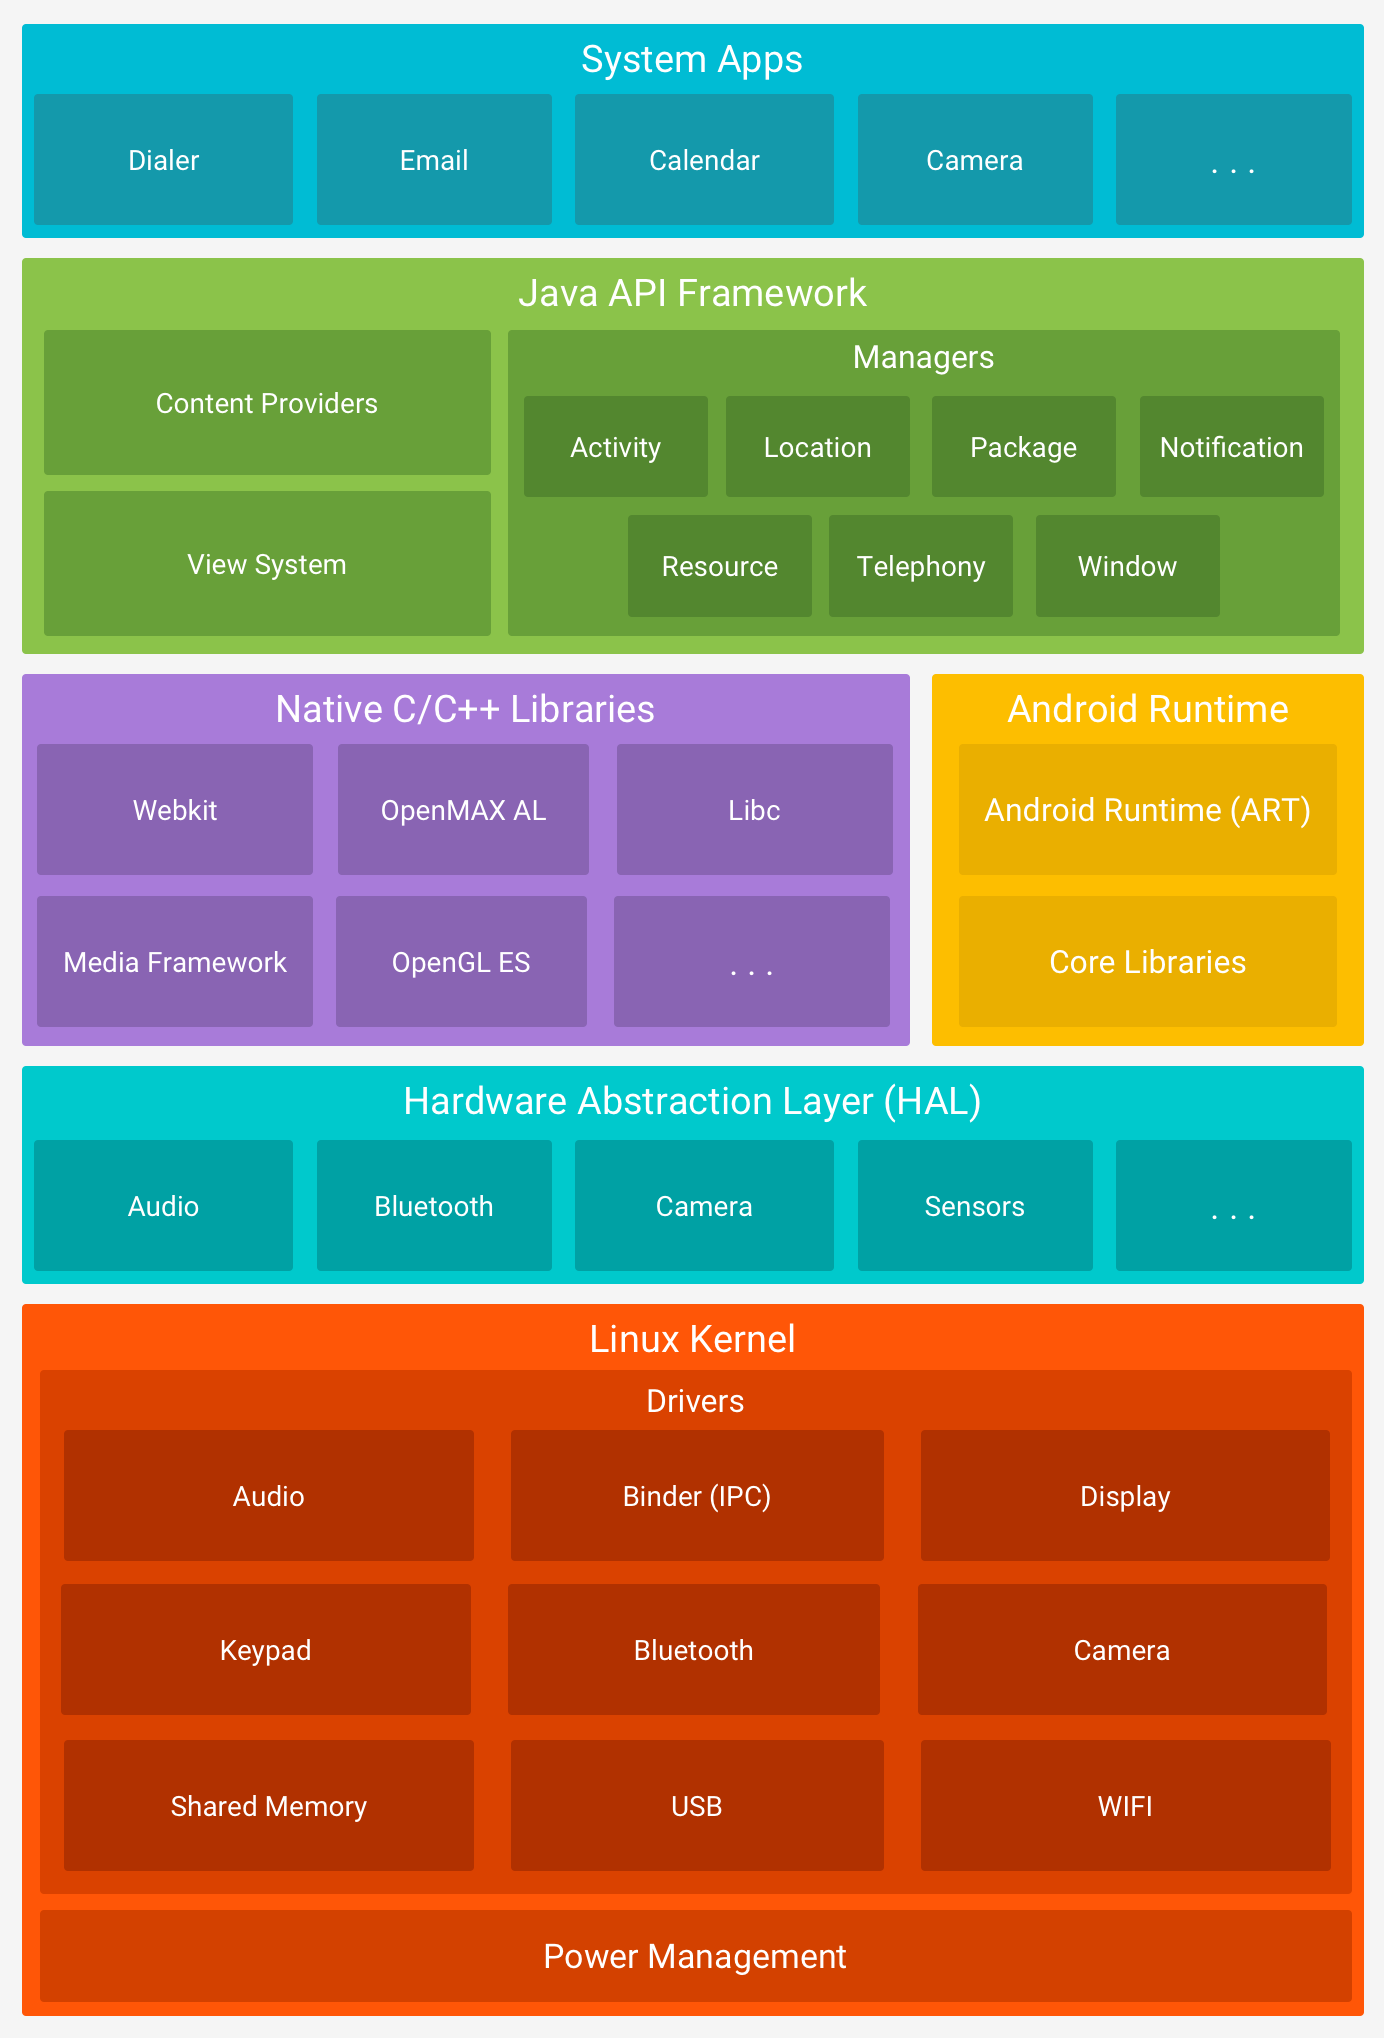
\includegraphics[width=0.7\textwidth]{bab2/figures/android-stack.png}
	\caption{Lapisan-lapisan pada Android}
	\label{fig:transfer-works}
\end{figure}

\section{Transfer Learning}
\par Transfer Learning adalah sebuah riset masalah pada pembelajaran mesin yang terfokus pada menyimpan pengetahuan yang didapat ketika menyelesaikan suatu masalah dan mengaplikasikannya ke masalah yang berbeda namun berhubungan \cite{transfer_def}. 
\begin{figure}[!ht]
	\centering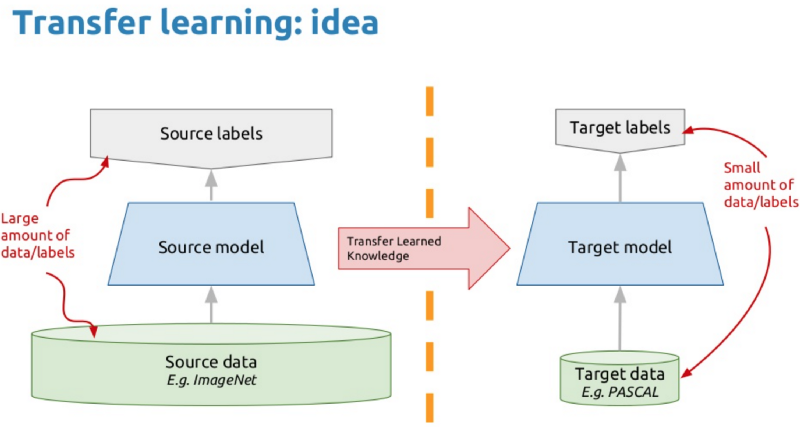
\includegraphics[width=0.7\textwidth]{bab2/figures/transfer-works.png}
	\caption{Diagram alir transfer learning\cite{transfer_pic}}
	\label{fig:transfer-works}
\end{figure}
\par Pendekatan Transfer Learning adalah dengan tiga metode, yaitu : 

\subsection{Melatih Sebuah Model untuk Menggunakannya Kembali}
\par Ketika kita ingin menyelesaikan Task A namun tidak memiliki cukup data untuk melatihnya dengan Deep Neural Network. Di sisi lain kita memiliki Task B dimana kita bisa melatihnya dengan Deep Neural Network. Maka kita dapat melatih Task B dengan Deep Neural Network dan menggunakannya sebagai titik awal dalam menyelesaikan Task A.

\subsection{Menggunakan Pre-Trained Model}
\par Pendekatan kedua adalah menggunakan dengan menggunakan pre-trained model atau model yang telah dilatih sebelumnya. Di internet banyak yang menyediakan pre-trained model ini, salah satunya Keras. Keras merupakan sebuah library pada Python yang menyediakan berbagai pre-trained model seperti VGG16, VGG19, XCeption, MobileNet dan lain-lain. 

\subsection{Ekstraksi Fitur}
\par Pendekatan lain adalah menggunakan algoritma \textit{Deep Learning} untuk menemukan representasi terbaik dari permasalahan. Pendekatan ini sering juga disebut \textit{Representation Learning}.  Cara menggunakan pendekatan ini adalah dengan menemukan fitur apa saja yang paling menggambarkan permasalahan kita. 
\par Meskipun metode Deep Learning dapat mengekstrak fitur secara otomatis, kita harus menentukan fitur mana saja yang ingin dimasukkan dalam \textit{Network}. Representasi yang sudah dipelajari kemudian dapat digunakan untuk menyelesaikan permasalahan lain juga. Metode ini cocok untuk menyelesaikan permasalahan Visi Komputer karena dapat mengurangi ukuran data set yang kemudian mengurangi waktu komputasi juga\cite{transfer_how}.

\begin{figure}[ht]
	\centering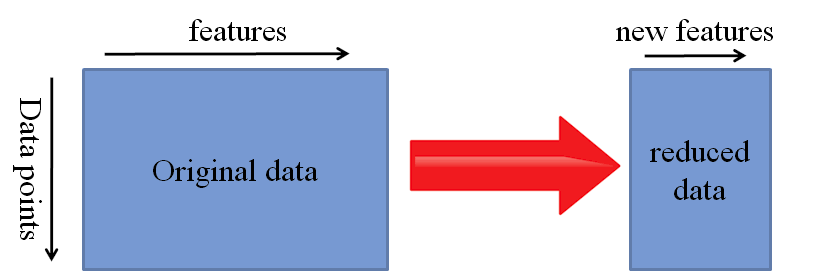
\includegraphics[width=0.7\textwidth]{bab2/figures/rep_features.png}
	\caption{Pembelajaran Representasi}
	\label{fig:rep-works}
\end{figure}

\section{Server}
\par \textit{Server} atau peladen dapat merujuk baik pada perangkat keras atau perangkat lunak yang menyediakan layanan akses kepada pengguna melalui protokol komunikasi HTTP atau HTTPS atas berkas-berkas yang terdapat pada suatu situs web dalam layanan ke pengguna dengan menggunakan aplikasi tertentu seperti peramban web \cite{webserver_def}.

\par Jika merujuk pada perangkat keras, web server digunakan untuk menyimpan semua data seperti HTML dokumen, gambar, file CSS stylesheets, dan file JavaScript. Sedangkan pada sisi perangkat lunak, fungsi web server adalah sebagai pusat kontrol untuk memproses permintaan yang diterima dari browser.

\par Secara sederhana, server bekerja atas permintaan dari sebuah klien. Misalnya saja untuk kasus web server, ketika Anda mengetikkan suatu alamat website menggunakan browser, maka artinya komputer Anda sedang bertindak sebagai klien yang meminta informasi kepada web server. Web server tersebut kemudian mengirimkan isi website ke komputer Anda, sehingga Anda pun dapat mengakses isi website tersebut.

\par Untuk kasus lainnya, seperti server FTP, mungkin agak sedikit berbeda. Pada server FTP, Anda dapat mengunggah sebuah dokumen atau data menuju server FTP, sehingga dapat disimpan dalam server tersebut. Sebagai klien, Anda berhak untuk menyimpan data Anda di server FTP. Nantinya, jika ada orang lain yang tergabung dalam jaringan server tersebut dan ingin mengunduh data atau dokumen Anda, maka server FTP akan menyediakan koneksi untuk klien lain tersebut.

\par Secara umum, semua jenis server bekerja dengan menjalankan fungsi-fungsi yang telah disebutkan sebelumnya, mulai dari melayani permintaan data dari klien hingga memberikan perlindungan pada komputer klien. Hanya saja, untuk jenis server yang berbeda, hal yang dilayani pun berbeda.

\par Sebuah perangkat komputer yang dijadikan server biasanya dirancang sedikit berbeda dari komputer – komputer klien. Dalam hal spesifikasi perangkat dan juga dalam hal sistem operasi misalnya, spesifikasi perangkat komputer yang digunakan sebagai server harus dibuat tinggi (karena harus menangani lalu lintas data yang cukup besar), sedangkan sistem operasinya harus menggunakan sistem operasi khusus server seperti Windows Server atau pun Linux Ubuntu Server / Linux Mint Server\cite{server_def}.

\section{Python}
\par Python adalah bahasa pemrograman yang populer. Python sering dimanfaatkan dalam pengembangan web, perangkat lunak, penelitian, dan system scripting. Python dapat digunakan untuk menangani data besar dan melakukan operasi matematika yang kompleks. Python bekerja di berbagai platform seperti Windows, Mac, Linux, Raspberry Pi, dan lain-lain. Python dirancang untuk mudah dibaca, yaitu memiliki sintaks yang sederhana dan
menggunakan bahasa Inggris\cite{python_def}.

\section{Tensorflow}
\par TensorFlow adalah library open source untuk pembuatan program yang membutuhkan komputasi numerik berkinerja tinggi. Dibuat oleh tim Google Brain, TensorFlow adalah librari \textit{open-source} untuk komputasi numerik dan pembelajaran mesin skala besar. TensorFlow menggabungkan satu set model dan algoritma pembelajaran mesin dan pembelajaran dalam (alias jaringan saraf) dan menjadikannya berguna melalui metafora umum. Tensorflow menggunakan Python untuk menyediakan API front-end yang nyaman untuk membangun aplikasi dengan kerangka kerja, sambil mengeksekusi aplikasi tersebut dalam C++.TensorFlow menyediakan fungsi-fungsi \textit{machine learning} dan \textit{deep learning}, dan dapat dijalankan dalam CPU atau GPU\cite{tensorflow_def}.

\section{Keras}
\par Keras adalah API neural network tingkat tinggi, ditulis dengan Python dan mampu berjalan di atas TensorFlow, CNTK, atau Theano. Keras dikembangkan dengan fokus pada mempercepat eksperimen\cite{keras_def}.
\par Keras tidak melakukan operasi tingkat rendahnya sendiri, seperti produk tensor dan konvolusi. Keras bergantung pada back-end. Meskipun Keras mendukung beberapa mesin back-end, back-end utamanya adalah TensorFlow, dan pendukung utamanya adalah Google. 
\par Keras API dikemas dalam TensorFlow sebagai tf.keras, yang seperti yang disebutkan sebelumnya akan menjadi TensorFlow API utama pada TensorFlow 2.0.

\section{VGG16}
\par VGG16 (juga disebut OxfordNet) adalah arsitektur jaringan saraf convolutional yang dinamai Grup Visual Geometry dari Oxford, yang mengembangkannya.[6] VGG16 terdiri dari 3 x 3 layer konvolusi, 2 x 2 max layer, dan fully-connected layer. Total layer pada VGG16 adalah 16\cite{vgg16_def}.

\section{VGG19}
\par VGG-19 adalah jaringan saraf convolutional yang dilatih pada lebih dari satu juta gambar dari database ImageNet. Jaringan ini memiliki 19 lapisan dan dapat mengklasifikasikan gambar ke dalam 1000 kategori objek, seperti keyboard, mouse, pensil, dan banyak binatang. Akibatnya, jaringan telah mempelajari representasi fitur yang kaya untuk berbagai gambar. Jaringan memiliki ukuran input gambar 224 x 224\cite{vgg19_def}.
\begin{figure}[!ht]
	\centering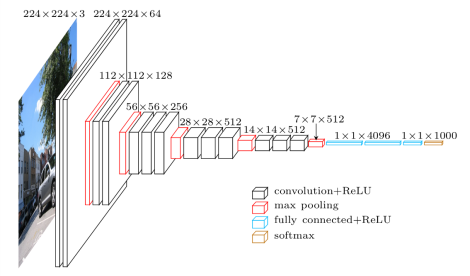
\includegraphics[width=0.7\textwidth]{bab2/figures/figure-vgg.png}
	\caption{Visualisasi dari arsitektur VGG\cite{figure_vgg}}
	\label{fig:abstraksi1}
\end{figure}

\section{MobileNet}
\par MobileNet didasarkan pada arsitektur ramping yang menggunakan konvolusi depth-wise terpisah untuk membangun jaringan saraf yang dalam dan ringan\cite{mobilenet_def}. 

\section{ResNet50}
\par ResNet adalah singkatan dari Residual Network. Residual dapat dipahami sebagai pengurangan fitur yang dipelajari dari input layer tersebut\cite{resnet_def}.

\section{Logistic Regression}
\par Logistic Regression digunakan dalam ilmu biologi pada awal abad kedua puluh. Itu kemudian digunakan dalam banyak aplikasi ilmu sosial. Logistic Regression digunakan ketika target adalah kategorikal\cite{logistic_def}.

\begin{figure}[!ht]
	\centering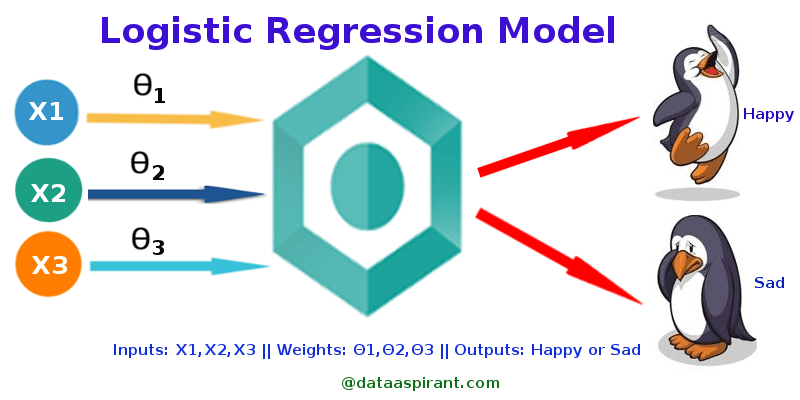
\includegraphics[width=0.7\textwidth]{bab2/figures/logistic.png}
	\caption{Visualisasi dari Logistic Regression}
	\label{fig:abstraksi1}
\end{figure}
\section{Precision}
\par Precision didefinisikan sebagai jumlah benar positif dibagi dengan jumlah benar positif ditambah jumlah salah positif. Salah positif adalah kasus-kasus yang oleh modelnya salah diberi label sebagai positif yang sebenarnya negatif\cite{precisionrecall}.

\section{Recall}
\par Recall adalah jumlah benar positif dibagi jumlah benar positif dibagi jumlah salah negatif \cite{precisionrecall}. Salah negatif menunjukkan nilai di mana kelas aktual adalah ya tetapi kelas prediksi adalah tidak. Misalnya, jika kelas aktual mengatakan bahwa akan hujan tetapi kelas prediksi menunjukkan bahwa tidak akan ada hujan.

\section{F1 Score}
\par Penghitungan F1 Score adalah dengan cara mengalikan dua dengan precision dan recall kemudian dibagi dengan penjumlahan precision dan recall. F1 Score mungkin merupakan ukuran yang lebih baik untuk digunakan jika kita perlu menemukan keseimbangan antara Precision dan Recall dan ada distribusi kelas yang tidak rata\cite{f1score_def}.